
\documentclass[11pt]{article} 

\usepackage[utf8]{inputenc} 
\usepackage{geometry} 
\geometry{a4paper} 

\vspace{2cm}
\setlength{\parindent}{0cm}
\usepackage{graphicx,wrapfig,placeins}

\title{Interactive Graphics}
\author{Chichi Francesco, Jary Pomponi}

\begin{document}
\maketitle
\graphicspath{{img/}}
\section{Introduction}
	The project developed from us is a local multi player game (1-4 players), inspired to the film \textit{Tron}.\\
	The goal of each player is to eliminate all the other players, and to do so, he have to traps them in some walls.
	When a player bump a wall or another player, he dies. At this point, the animation of the death start, and when it's ended, the ship and the relative walls disappear from the map.
\section{List of all the libraries, tools and models used in the project but	not developed by the team}
\begin{itemize}
	\item \textbf{Three.js:}
		Three.js is a cross-browser JavaScript library/API used to create and display animated 3D computer graphics in a web browser exploiting the power of WebGL in an high level mode.
	\item \textbf{OrbitControls.js:}
		We used OrbitControls to allow the user to move the camera in the space.
	\item \textbf{Detector.js:}
		Detector is necessary to verify if the user's browser support \textit{WebGL}.
	\item \textbf{stats.min.js:}
		stats.min is used to show the FPS, frame per second, or the MS, the millisecond used for each render.
		
\end{itemize}
\section{Description of all the technical aspects of the project}
\subsection{Ship}
	
	
	\begin{wrapfigure}{R}{0pt}
		\centering
		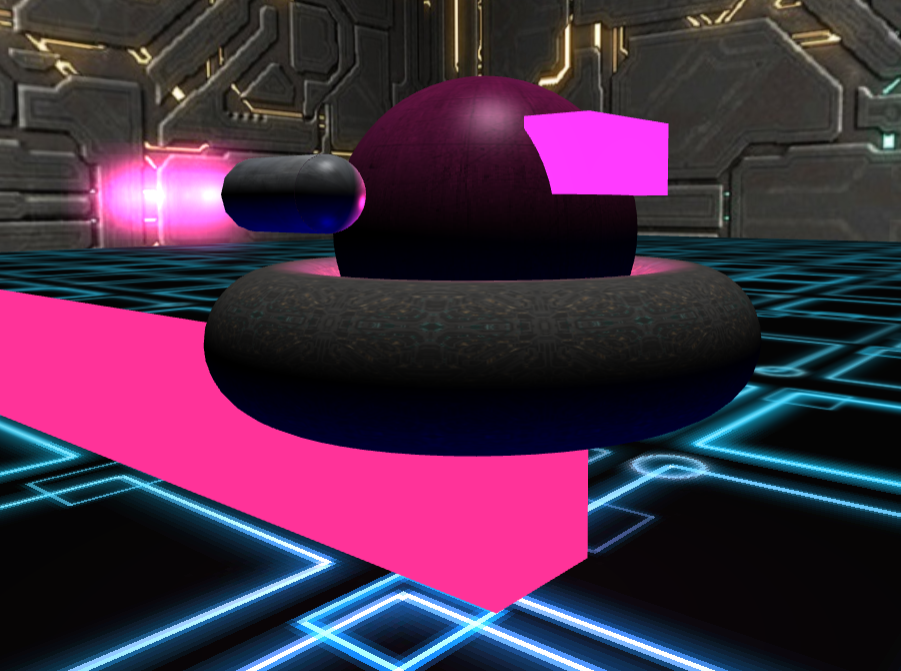
\includegraphics[width=0.4\linewidth]{ship}
		\caption{This is the character of a player that choosen the pink colour.}
		\label{fig:ship}
	\end{wrapfigure}
	
	Each player has a ship of the choosen colour, which one is a three.js Group, composed by a \textbf{cabin} (fig. 2), a clock wise rotating \textbf{ring} (fig. 3) and two \textbf{motors} (fig. 4).\\
	
	The cabin is also a Group of element coloured with the player's colour, composed by a glass and a cockpit with a pointlight inside.
	The cockpit is a sphere covered with a metallic texture, the glass is a parallelepiped made by a \textit{MeshToonMaterial}, that is illuminated by the cockpit's light.\\
	
	Each motor is another independent Group, composed by a cylinder, an hemisphere on the top and another hemisphere with an hole, that represent the exhaust pipe, each one is covered with the metallic texture of the cabin.
	Furthermore, at the end of the exhaust pipe, there are 50 particles of the colour of the player. The wake's length where this particles are distributed is choosen stochastically: with a probability of 80\%, the wake's length is equal to 40, with 10\% is 0 or 10.\\
	
	Finally, there is a rotating ring, that is a torus coloured with the same texture of the torus which rotates around the map.
	
	\begin{figure}
		\centering
		\begin{minipage}[b]{0.25\linewidth}
			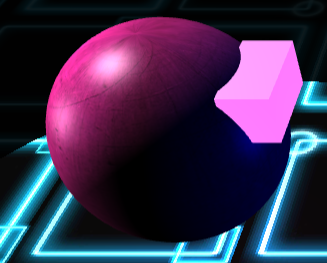
\includegraphics[width=\linewidth]{cabin}
			\caption{The cabin of the ship.}
			\label{fig:cabin}
		\end{minipage}
		\begin{minipage}[b]{0.276\linewidth}
			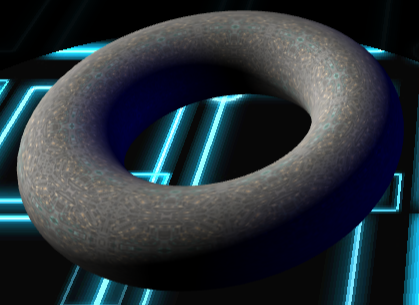
\includegraphics[width=\linewidth]{toro}
			\caption{The rotating torus.}
			\label{fig:toro}
		\end{minipage}
		\begin{minipage}[b]{0.6\linewidth}
			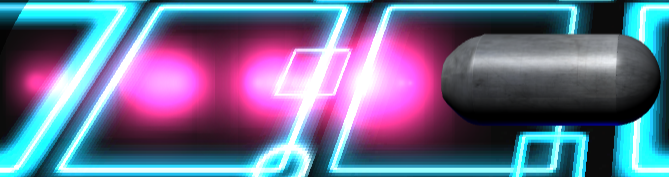
\includegraphics[width=\linewidth]{motor}
			\caption{A motor with the particles.}
			\label{fig:motor}
		\end{minipage}
	\end{figure}





\subsection{Halo}
\subsection{Animated Light}
\subsection{Collision}
\subsection{Menu}
	The game contains several menu views: The \textbf{main menu} (fig. ), \textbf{key settings} (fig. ), \textbf{colour settings} (fig. ), \textbf{end game} (fig. ), \textbf{pause} (fig. ).\\
	
	The main menu allow the users to start the game, to go in the key settings menu or to the colour settings menu.
	Furthermore, it allow to change the principal settings of the game: choose the number of playing players, decide if allow the main soundtrack and the in-game sound effect, only the last one or to play without any kind of sounds, and finally to choose between the three light modalities, \textbf{day}, \textbf{night} or \textbf{cycle}.\\
	Next to the main menu, there are a view of all the 4 ships, below there is a pillar representing the ranking position of the relative player (fig. ).
	Furthermore, the first ranked player is lit up by a spotlight.\\
	
	The key settings menu is used in order to modify the default value of the command for each player. In the menu is shown, fore each player, the relative number of the player with the choosen colour and two button, usable to change the \textit{turn-left} and \textit{turn-right} commands values.\\
	
	In the colour setting menu we can find three slider fore each player, relative to the RGB colour, and a bar coloured with the result of the three component.\\
	On the left of this menu are showed the four ships with their choosen relative colors.
	
	When only one player still alive, if the initial number of player was at least 2, the end game menu is showed, in which we find a table showing the ranking of the players in game. In this table there are the numbers relative of each player, if the colour is grey, it means that the relative player is not playing, otherwise are shown the colours relative to the player.
	Furthermore, in the same menu are shown two button, one to come back to main menu, other to play again the game.\\
	
	Finally there is a pause menu, where we can find three buttons: the same two button described in the end game menu and another one to show the key settings menu.\\
	 
\begin{figure}
	\centering
	\begin{minipage}[b]{0.3005\linewidth}
		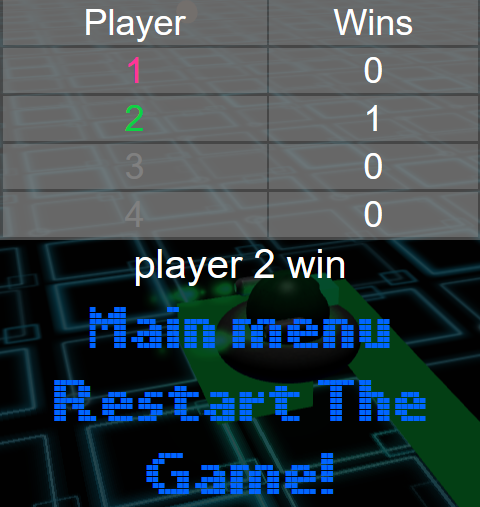
\includegraphics[width=\linewidth]{endGameMenu2}
		\caption{with 2 player}
		\label{fig:endGameMenu2}
	\end{minipage}
	\begin{minipage}[b]{0.3015\linewidth}
		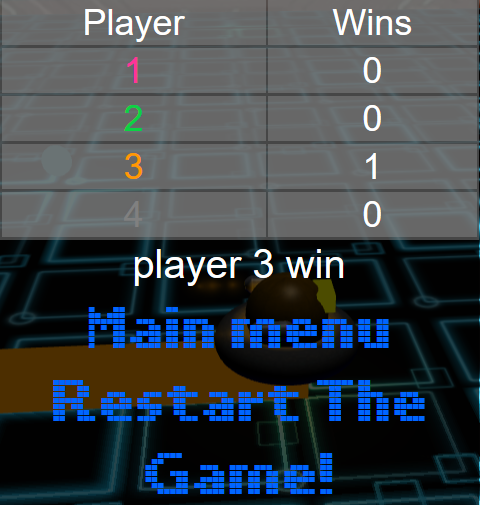
\includegraphics[width=\linewidth]{endGameMenu3}
		\caption{with 3 player}
		\label{fig:endGameMenu3}
	\end{minipage}
	\begin{minipage}[b]{0.2955\linewidth}
		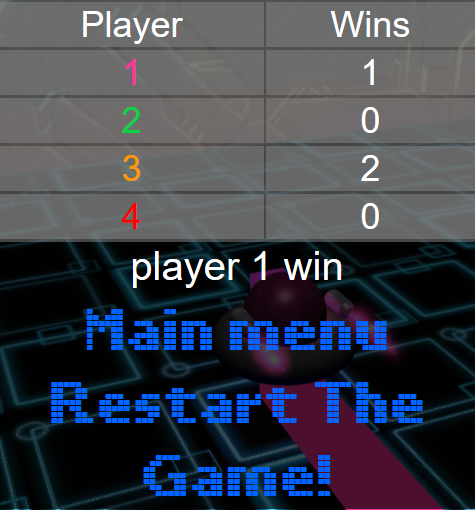
\includegraphics[width=\linewidth]{endGameMenu4}
		\caption{with 4 player}
		\label{fig:endGameMenu4}
	\end{minipage}
\end{figure}

\begin{figure}
	\centering
	\begin{minipage}[b]{0.3\linewidth}
		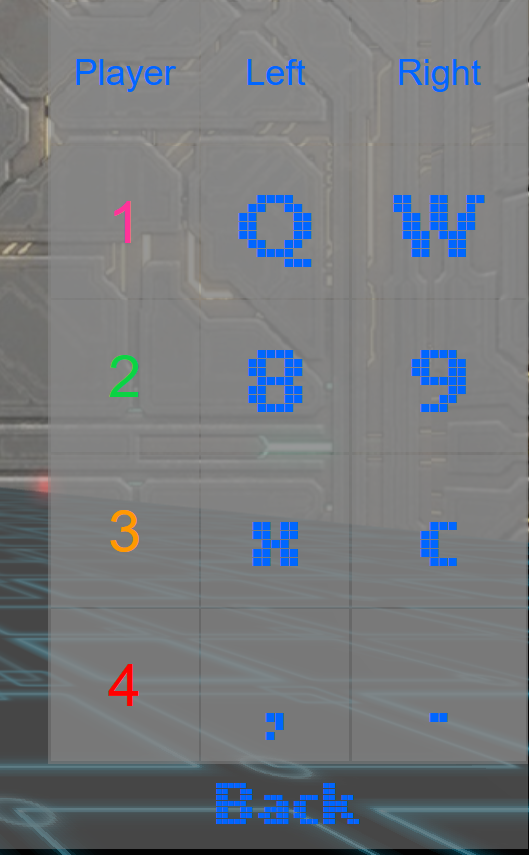
\includegraphics[width=\linewidth]{keySettingsMenu}
		\caption{This is the menu used to change the default controls value.}
		\label{fig:keySett}
	\end{minipage}
	\begin{minipage}[b]{0.32\linewidth}
		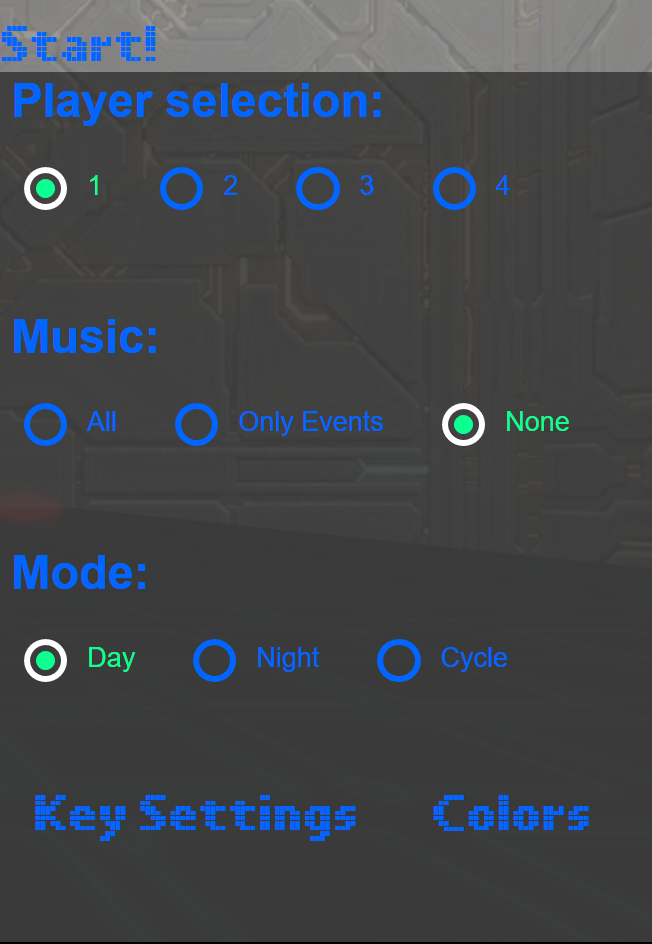
\includegraphics[width=\linewidth]{startMenu}
		\caption{This is the main menu, used to start the game or to change some of the principal settings.}
		\label{fig:startMenu}
	\end{minipage}
	\begin{minipage}[b]{0.3\linewidth}
		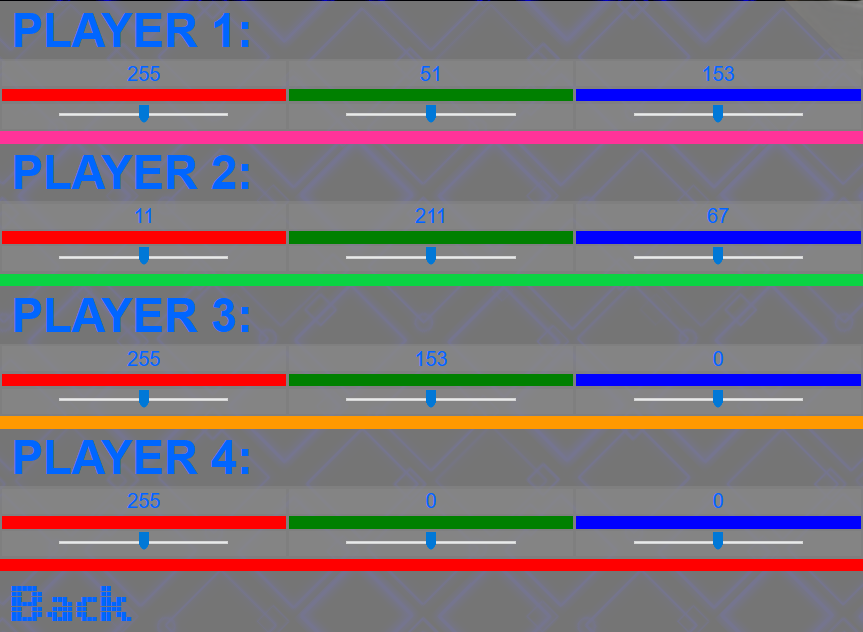
\includegraphics[width=\linewidth]{colorMenu}
		\caption{This is the menu used to change the default colours value.}
		\label{fig:colorMenu}
	\end{minipage}
	\begin{minipage}[b]{0.6\linewidth}
		
\includegraphics[width=\linewidth]{pauseMenu}
		\caption{This is the pause menu}
		\label{fig:endGameMenu4}
	\end{minipage}
	\begin{minipage}[b]{0.6\linewidth}
		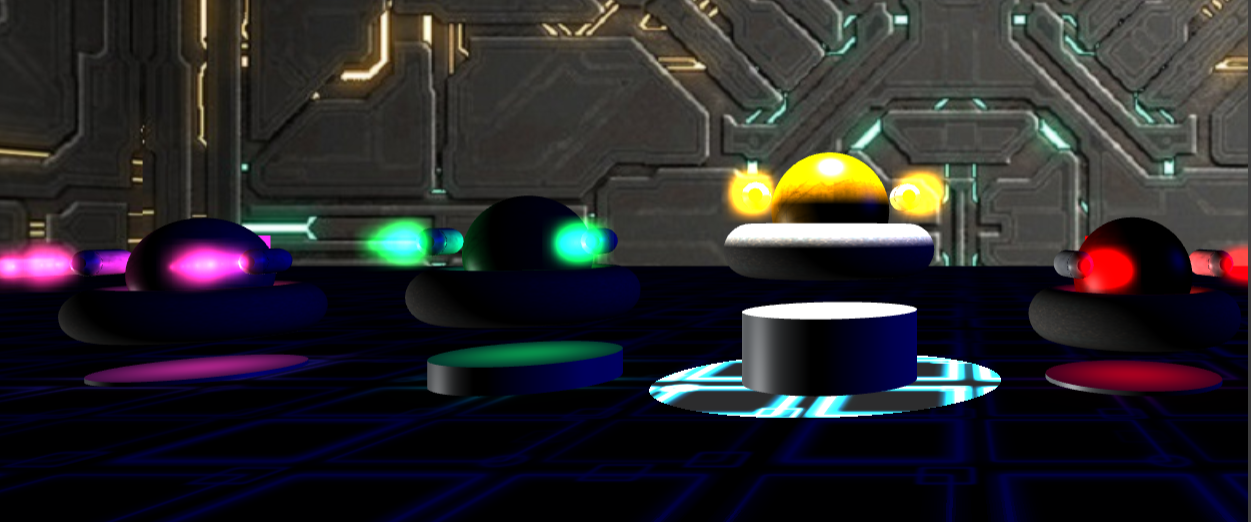
\includegraphics[width=\linewidth]{Ranking}
		\caption{This is the ranking shown in the main menu.}
		\label{fig:Ranking}
	\end{minipage}
\end{figure}

\section{Description of the implemented interactions}

\end{document}
